%%%%%%%%%%%%%%%%%%%%%%%%%%%%%%%%%%%%%%%%%
% Simple Sectioned Essay Template
% LaTeX Template
%
% This template has been downloaded from:
% http://www.latextemplates.com
%
% Note:
% The \lipsum[#] commands throughout this template generate dummy text
% to fill the template out. These commands should all be removed when 
% writing essay content.
%
%%%%%%%%%%%%%%%%%%%%%%%%%%%%%%%%%%%%%%%%%

%----------------------------------------------------------------------------------------
%	PACKAGES AND OTHER DOCUMENT CONFIGURATIONS
%----------------------------------------------------------------------------------------
\documentclass[12pt]{article} % Default font size is 12pt, it can be changed here

\usepackage{geometry} % Required to change the page size to A4
\geometry{a4paper} % Set the page size to be A4 as opposed to the default US Letter

\usepackage{graphicx} % Required for including pictures

\usepackage{float} % Allows putting an [H] in \begin{figure} to specify the exact location of the figure

\usepackage{amsmath}
\usepackage{amssymb}


\usepackage{graphicx}
\usepackage{subcaption}

\usepackage{float}
\restylefloat{table}

\usepackage{tabu}

\linespread{1.2} % Line spacing

%\setlength\parindent{0pt} % Uncomment to remove all indentation from paragraphs

\graphicspath{{Pictures/}} % Specifies the directory where pictures are stored

\usepackage[
    backend=biber,
    style=ieee
]{biblatex}
\addbibresource{bibliography.bib}

\usepackage[]{hyperref}
\usepackage{cleveref}


\begin{document}

%----------------------------------------------------------------------------------------
%	TITLE PAGE
%----------------------------------------------------------------------------------------

\begin{titlepage}

\newcommand{\HRule}{\rule{\linewidth}{0.5mm}} % Defines a new command for the horizontal lines, change thickness here

\center % Center everything on the page

\textsc{\LARGE University of York}\\[1.5cm] % Name of your university/college
\textsc{\Large MLAP}\\[0.5cm] % Major heading such as course name
\textsc{\large Machine Learning and Applications}\\[0.5cm] % Minor heading such as course title

\HRule \\[0.4cm]
{ \huge \bfseries Open Examination}\\[0.4cm] % Title of your document
\HRule \\[1.5cm]

\begin{minipage}{0.4\textwidth}
\begin{flushleft} \large
\center \emph{Examination number:}\\
\center Y3606797
\end{flushleft}
\end{minipage}

%\includegraphics{Logo}\\[1cm] % Include a department/university logo - this will require the graphicx package

\vfill % Fill the rest of the page with whitespace

\end{titlepage}

%----------------------------------------------------------------------------------------
%	TABLE OF CONTENTS
%----------------------------------------------------------------------------------------

\tableofcontents % Include a table of contents

\newpage % Begins the essay on a new page instead of on the same page as the table of contents 

%----------------------------------------------------------------------------------------
%	INTRODUCTION
%----------------------------------------------------------------------------------------

\section{Task 1} % Major section

%------------------------------------------------

\subsection{What sort of model?} % Sub-section
The naive Bayes model makes the assumption that all features are conditionally independent given the class. The given Bayesian network explicitly models the conditional independence in it's structure.

\subsection{EM in general}
The EM algorithm is an iterative approach to maximising the likelihood when we have hidden variables. We have a model $p(\upsilon,h|\theta)$ and we wish to find $\theta$ by maximising the marginal likelihood $p(\upsilon|\theta)$. EM achieves this by replacing the marginal likelihood with a lower bound, the bound depends on $\theta$ and the set of variational distributions $\{q\}$, we optimise this bound. This is done by first fixing $\theta$ and then optimising \textit{w.r.t} $\{q\}$, then fixing $\{q\}$ and optimising \textit{w.r.t} $\theta$. These are known as the 'E' and 'M' steps and are repeated until convergence. The EM algorithm may not always return the correct MLEs because it can get stuck on local optima.

\subsection{EM for the current model}
Firstly we assume some initial parameters for the distribution, so we have $\theta_{X1}^0$, $\theta_{X2}^0$, $\theta_{X3}^0$, $\theta_{H}^0$ and $\theta_{C}^0$. Then we compute the distribution for the hidden data H:
$$
q_{t=1}^{n=1}(H)=p(H|C=0,X1=0,X2=0,X3=1,\theta^0),
$$
$$
q_{t=1}^{n=2}(H)=p(H|C=1,X1=1,X2=0,X3=0,\theta^0)...
$$
and so on for each data point in the training data. This is first E-step in the algorithm.

The first M-step involves maximising the energy term by choosing new values for $\theta$. The energy term is given by the following equation:
\begin{multline}
E(\theta) = \displaystyle\sum_{n=1}^{N}
\{
\langle\log p(C^n|H^n) \rangle_{q_t^n(H)} +
\langle\log p(X1^n|H^n) \rangle_{q_t^n(H)} + 
\langle\log p(X2^n|H^n) \rangle_{q_t^n(H)} \\ +
\langle\log p(X3^n|H^n) \rangle_{q_t^n(H)} + 
\langle\log p(H^n) \rangle_{q_t^n(H)}
\}
\end{multline}

To calculate the M-step update for each table we have to maximise each term of the above equation individually. The contribution of the term $p(C=i|H=j)$ is given by:
$$
\displaystyle\sum_{n}\mathbb{I}[C^n=i]q^n(H=j) \log p(C=i|H=j))
$$
where the indicator function $\mathbb{I}[C^n=i]$ equals 1 if C is in state i and is zero otherwise.
We normalise the table by adding a Lagrange term:
$$
\displaystyle\sum_{n}\mathbb{I}[C^n=i]q^n(H=j) \log p(C=i|H=j))
+ \lambda\{1-\sum_{k}p(C=k|H=j)\}
$$
We differentiate with respect to $p(C=i|H=j)$ and equate to zero to find the maximum, this gives us:
$$
\displaystyle\sum_{n}\mathbb{I}[C^n=i] \frac{q^n(H=j)}{p(C=i|H=j)} = \lambda
$$
Hence
$$
p(C=i|H=j)=
\frac{\sum_{n}\mathbb{I}[C^n=i]q^n(H=j)}{\sum_{n,k}\mathbb{I}[C^n=k]q^n(H=j)}
$$
This result highlights a relationship between the table updates and the standard MLE. That is, when we have missing data we replace the functions such as $\mathbb{I}[C^n=i]$ which represent the real counts of the data, by the assumed distributions $q$. We use this relationship to calculate the table updates for each other term in the energy equation.

We can then perform the E-step again using our updated parameters such that we have new assumed distributions for the hidden variable:
$$
q_{t}^{n=1}(H)=p(H|C=0,X1=0,X2=0,X3=1,\theta^{t-1}),
$$
$$
q_{t}^{n=2}(H)=p(H|C=1,X1=1,X2=0,X3=0,\theta^{t-1})...
$$
We perform the steps E and M iteratively until the algorithm converges to a local optima.

\subsection{Gibbs sampling for the current model}
We start by initially setting the 'state' of the variables to some values, usually according to their prior distributions. Then we pick a variable, C for example, and sample from it's conditional distribution.

From Bayes theorem:
$$
P(X1,X2,X3,C,H)=
P(C|X1,X2,X3,H)
P(X1,X2,X3,H)
$$
We could sample from the following distribution:
$$
P(C|X1,X2,X3,H)
$$
But we only need to take into account the values of the variables within the currently sampled variables Markov blanket, as defined by the nodes in the BN which are the parent, child or co-parents of the current node.

Hence we can sample from: $P(C|H)/Z$ where Z is a normalisation factor. We update the variable value to the sample in a new instance of the 'state' and we repeat for the remaining variables.

The theory of MCMC guarantees that the stationary distribution of the samples generated by Gibbs sampling will be an approximation of the joint posterior distribution for a large enough number of samples.

\subsection{Running Gibbs sampling for the current model}
I ran the sampler for 1000 iterations as a burn in, this was done to essentially discard initial samples that may not be representative of the stationary distribution. I then ran around 500000 iterations to converge on the distribution.

The kernel density distribution in \cref{fig:H Posterior} represents the approximate distribution for the hidden variable H. The shape resembles the uniform distribution which means that the two possible values for H are approximately equally probable.

\subsubsection{Compare contrast EM/Gibbs sampling}
A downside to Gibbs sampling is that the samples are very dependent given the previous samples, due to the nature of MCMC. A downside of EM is that is can get stuck on local optima and not return the true maximum value for the parameters. Similarly for Gibbs sampling it is unknown how many iterations are required for convergence.

In the Bayesian approach we also have the option to incorporate informative priors into our learning, which increases the accuracy of our results, but can also complicate them. Both approaches are fairly easy computationally which is why they are popular methods for inference problems.

\begin{table}[h!]
\centering
\begin{tabu} to 0.8\textwidth { | X[l] | X[l] | X[l] | }
 \hline
 parameter & mean & sd \\
 \hline
 h.theta[1] & 0.4991 & 0.2907 \\
 \hline
 h.theta[2] & 0.5009  & 0.2907 \\
 \hline
 c.theta[1,1] & 0.5008 & 0.2674 \\
 \hline
 c.theta[1,2] & 0.4992  & 0.2674 \\
  \hline
 c.theta[2,1] & 0.4984  & 0.2671 \\
  \hline
 c.theta[2,2] & 0.5016  & 0.2671 \\
 \hline
 x1.theta[1,1] & 0.5015 & 0.2671 \\
 \hline
 x1.theta[1,2] & 0.4985  & 0.2671 \\
  \hline
 x1.theta[2,1] & 0.4985  & 0.2668 \\
  \hline
 x1.theta[2,2] & 0.5015  & 0.2668 \\
 \hline
 x2.theta[1,1] & 0.708 & 0.2445 \\
 \hline
 x2.theta[1,2] & 0.292  & 0.2445 \\
  \hline
 x2.theta[2,1] & 0.7088  & 0.244 \\
  \hline
 x2.theta[2,2] & 0.2912  & 0.244 \\
 \hline
 x3.theta[1,1] & 0.708 & 0.2445 \\
 \hline
 x3.theta[1,2] & 0.292  & 0.2445 \\
  \hline
 x3.theta[2,1] & 0.709  & 0.2445 \\
  \hline
 x3.theta[2,2] & 0.291  & 0.2445 \\
\hline
\end{tabu}
\end{table}

\begin{figure}[h!]
  \centering
  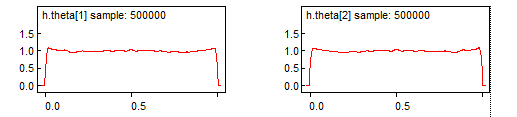
\includegraphics[width=\linewidth]{bugs_graphs/h.png}
  \caption{Approximate posterior distribution for H}
  \label{fig:H Posterior}
\end{figure}

\begin{figure}[h!]
  \centering
  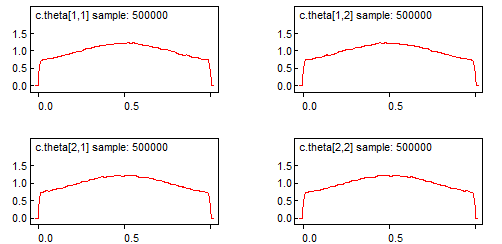
\includegraphics[width=\linewidth]{bugs_graphs/c.png}
  \caption{Approximate posterior distribution for C}
  \label{fig:C Posterior}
\end{figure}

\begin{figure}[h!]
  \centering
  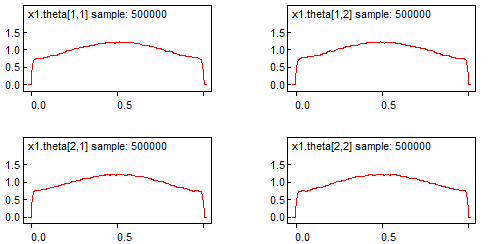
\includegraphics[width=\linewidth]{bugs_graphs/x1.png}
  \caption{Approximate posterior distribution for X1}
  \label{fig:X1 Posterior}
\end{figure}

\begin{figure}[h!]
  \centering
  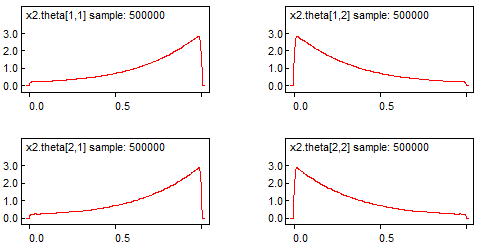
\includegraphics[width=\linewidth]{bugs_graphs/x2.png}
  \caption{Approximate posterior distribution for X2}
  \label{fig:X2 Posterior}
\end{figure}

\begin{figure}[h!]
  \centering
  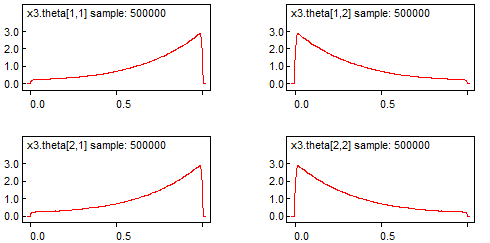
\includegraphics[width=\linewidth]{bugs_graphs/x3.png}
  \caption{Approximate posterior distribution for X3}
  \label{fig:X3 Posterior}
\end{figure}

\clearpage

\subsection{Using informative priors}

I edited the prior for variables H and C to express that they were both highly likely to be the same value, the result of this can be seen in \cref{fig:H_2 Posterior} and \cref{fig:C_2 Posterior}.

This change resulted in completely different shapes for the estimate distributions of the posteriors for variables X1, X2 and X3 as seen in \cref{fig:X1_2 Posterior}, \cref{fig:X2_2 Posterior} and \cref{fig:X3_2 Posterior}. H and C now obviously tend towards the more probable values for the variables as defined by my chosen prior.

The values of the variables X1, X2, and X3 now seem to be more evenly distributed for the improbable value of H, they resemble uniform distributions (slightly skewed for X2 and X3). The values of X1, X2 and X3 seem to remain biased against the probable value of H under these prior assumptions.

\begin{figure}[h!]
  \centering
  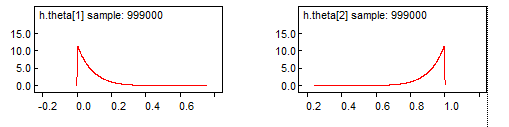
\includegraphics[width=\linewidth]{bugs_graphs/h_2.png}
  \caption{Approximate posterior distribution for H with informative prior}
  \label{fig:H_2 Posterior}
\end{figure}

\begin{figure}[h!]
  \centering
  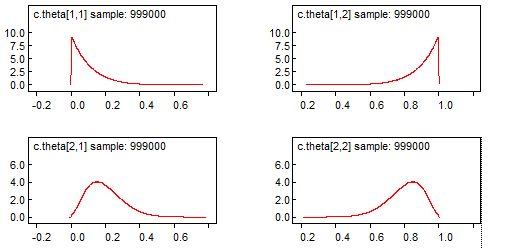
\includegraphics[width=\linewidth]{bugs_graphs/c_2.png}
  \caption{Approximate posterior distribution for C with informative prior}
  \label{fig:C_2 Posterior}
\end{figure}

\begin{figure}[h!]
  \centering
  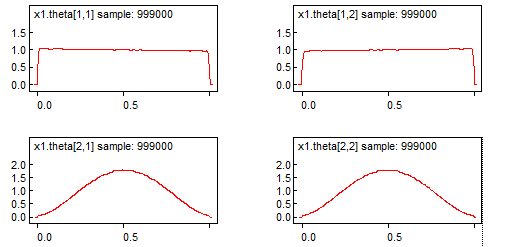
\includegraphics[width=\linewidth]{bugs_graphs/x1_2.png}
  \caption{Approximate posterior distribution for X1}
  \label{fig:X1_2 Posterior}
\end{figure}

\begin{figure}[h!]
  \centering
  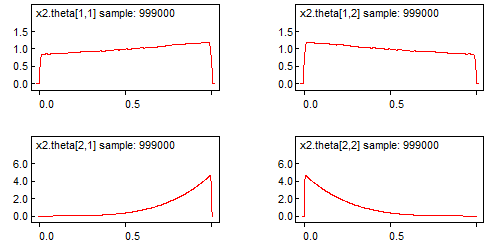
\includegraphics[width=\linewidth]{bugs_graphs/x2_2.png}
  \caption{Approximate posterior distribution for X2}
  \label{fig:X2_2 Posterior}
\end{figure}

\begin{figure}[h!]
  \centering
  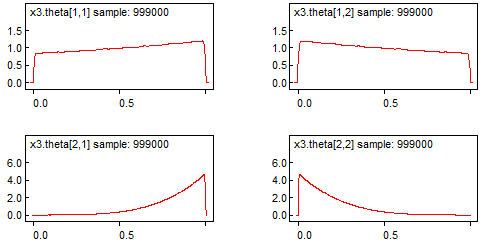
\includegraphics[width=\linewidth]{bugs_graphs/x3_2.png}
  \caption{Approximate posterior distribution for X3}
  \label{fig:X3_2 Posterior}
\end{figure}

\clearpage

\printbibliography 
\end{document}